\documentclass[conference]{IEEEtran}

  \usepackage{booktabs}
  \usepackage{listing}
  \usepackage{amsmath}
  \usepackage{algorithm}
  \usepackage{array}
  \usepackage{url}
  \usepackage{cite}
  \usepackage{complexity}
  \usepackage{algpseudocode}
   \usepackage{graphicx}
% \usepackage{algorithm}
  \ifCLASSINFOpdf
  
  \else
  
  \fi
  
  \hyphenation{op-tical net-works semi-conduc-tor}
  
  
  \begin{document}
  
  \title{Parallel Distributed Multi-objective Fuzzy Genetics-based Machine Learning \\ Mid Term Report}
  
  \author{\IEEEauthorblockN{Bowen Zheng, Shijie Chen, Shuxin Wang}
  \IEEEauthorblockA{Department of Computer Science and Engineering\\
  Southern University of Science and Technology\\
  Shenzhen, Guangdong, China\\}
  }
  
  \maketitle
  
  \begin{abstract}
  In the second period of the project, we finished the design of fuzzy classifiers, GBML framework and the asynchronous parallel distributed system. We have implemented each part respectively and are working to integrate them together.
  \end{abstract}
  \IEEEpeerreviewmaketitle
  
  \section{Introduction}
  In this project, we aim to build a parallel distributed implementation of a multi-objective genetics based machine learning(GBML) algorithm. We choose a specific problem of a three-objective fuzzy rule-based classifier and fit it into a hybrid GBML framework. Then we develop a parallel mechanism to accelerate computation.

  Code of the three parts have been completed. We will integrate them together, fix bugs and run some test problems in the next stage.

  \section{Fuzzy Rule-based Classifiers}
  The design and implementation of fuzzy classifier is based on \cite{ishibuchi2007analysis}.
  \subsection{Fuzzy Rules}
  \subsection{Fuzzy Classifier}

  \section{Hybrid Genetics-based Machine Learning Framework}
	 \par After designing the fuzzy classifier, the next step is approaching our three objectives: correctly classified training patterns, number of fuzzy rules and total number of antecedent conditions in the fuzzy classifier S.
	 \par
	 We use a hybrid GBML algorithm to find the non-dominated rule sets of this problem. The genetic algorithm we used is basically following \cite{ISHIBUCHI20074}. This hybrid GBML is implemented in the framework of non-dominated sorting genetic algorithm II(NSGA-II) and it's a Pittsburgh-style algorithm. Besides, it use Michigan-style GBML to change a rule as the mutation operation. 
	 \par
	In our genetic algorithm, the population is a set of fuzzy classifier, and the individual is a single fuzzy classifier (i.e., a set of fuzzy rules). The basic steps of our algorithm is followed. First step, we'll initialize our population with size $N_pop$ using training data. Second step, we'll generate $N_pop$ offspring by implementing selecting and crossover operators to two parents, and do mutate on the offspring. Third step, the origin and offspring population will be combined together and we only keep the first $N_pop$ individuals after the population sorting by Pareto ranking and crowding measure, which will be introduced later. Finally, we'll check whether it have reached the stop condition,and if not we'll go back to the second step.
	 
	 \subsection{NSGA-II}
	 \par
	 NSGA-II is introduced detailedly in \cite{996017}, which is a common algorithm in multi-objective optimizing problem. I think the characters of NSGA-II algorithm comparing with a ordinary genetic algorithm is that it uses elite-preserving, Pareto ranking, and crowding measure. Elite-preserving is a strategy that can reserve outstanding gene by keeping the individual containing such a gene. Pareto ranking and crowding measure is used to compare individuals in the three-objective situation. We'll introduce the three futures respectively.
	 \subsubsection{Elite-preserving}
	 \par
	 Elite-preserving is a replacing strategy at the end of a generation. The basic idea is that we only replace individuals with bad performance in original population by the outstanding offspring, and we keep preeminent parents to reserve their high performance gene. And we measure individuals' performances using Pareto ranking and crowding measure.
	 
	 
	 \subsubsection{Pareto ranking}
	 \par
	 Pareto-optimal front is the solution set that we want to find in the multi-objective optimizing problem, and its definition can been seen at \cite{ISHIBUCHI20074}. In the multi-objective optimizing problem, individual in Pareto-optimal front can be seen as the "best" solution. We'll give these individuals the highest Pareto ranking. If we remove the individuals in Pareto-optimal front, we can find another Pareto-optimal front of the remaining individuals. Then we'll give the second front a lower Pareto ranking than previous one, and we continue do such iteration until every individual gets their Pareto ranking. And we can measure individuals' performance by their Pareto ranking. If individuals have same ranking number, we'll compare them by using crowding measure.
	 
	 \subsubsection{Crowding measure}
	 \par
	 Crowding measure can help us finding a more diverse Pareto set. As we wanting to find a more homogeneous solutions set, we'd like to choose the individual in a less crowded area. To estimate the density of a individual in a population, we calculate the sum of the distances to neighbor individuals on both side and for each objective. And shorter the distance is, more crowded area the individual is in.     
	 
	 \subsection{Michigan-style GBML}
	 \par
	 Different Pittsburgh-style algorithm, Michigan-style GBML see a single fuzzy rule as a population and see the membership function as an individual. So we use Michigan-style GBML as a mutation operator acting on a single rule to enrich the diversity of our population. 
	 \subsection{Validation}
	 After implementing our program, we validate its reliability using iris data set and it have successfully pass the feasibility test. The results are followed.
	 \\
	 \begin{tabular}{cccccc}
	 	\hline
	 	Number of rules& 1& 2&3&4&5\\
	 	\hline
	 	NO. of correctly classified pattern& 49& 99&132&134&137\\
	 	\hline
	 	error rate&0.67&0.34&0.12&0.11&0.09\\
	 	\hline
	 \end{tabular}

 \begin{figure}[H]
 	\centering
 	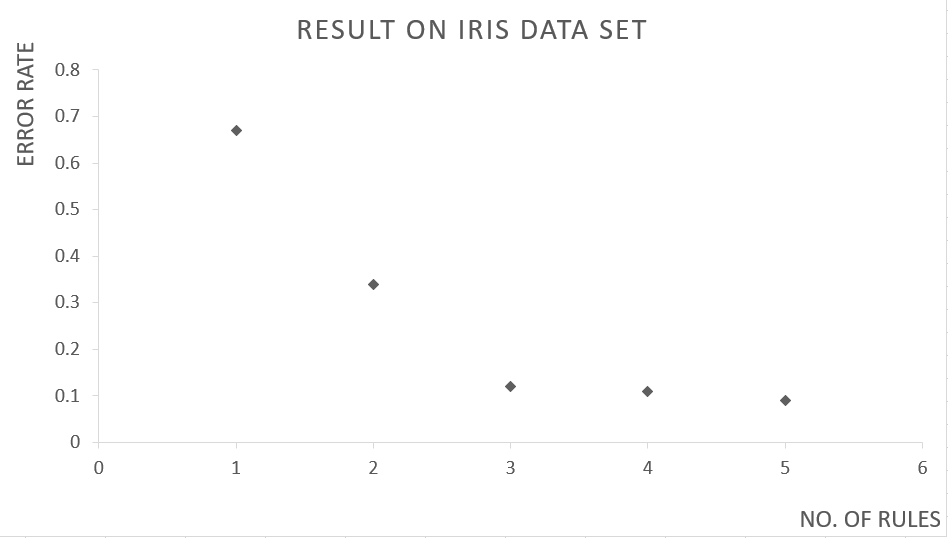
\includegraphics[width=0.5\textwidth]{iris.png}
 	\caption{Handwrite}\label{fig:digit}
 \end{figure}
  \section{Asynchronous Parallel Distributed System Design}


  \section{Contribution}
    \begin{itemize}
    \item Bowen Zheng - Design \& Implementation of parallel system
    \item Shijie Chen - Design \& Implementation of fuzzy classifier, Design of parallel system
    \item Shuxin Wang - Design \& Implementation of Hybrid GBML framework
    \end{itemize}
    

  \section*{Acknowledgment}


\bibliographystyle{ieeetr}
\bibliography{ref}
% that's all folks
\end{document}


  